\section{Modeller}

Her følger uformell dokumentasjon over dataevolusjonsmoculen DBUpgradinator og hvordan den skal oppføre seg i en datadreven webapplikasjon hvis dataelementer persisteres i en distribuert database. Dokumentasjonen er basert på 4+1-metamodellen Phillippe Kruchten presenterer i en artikkel fra 1995.

\subsection{4+1 - stilen}

Dokumentasjon av programvarearkitektur er en kommunikasjonskunst. Symbolene som tegnes på et lerret eller på en bildefil bærer ingen betydning eller mening i seg selv, hva de representerer er noe dokumentets forfattere og dets påtenkte publikum må være samstemte om. Videre er tydelige kommuniserende begrenset når det kommer til hvor mange konsepter de kan representere på ett og samme tidspunkt. En firkant, eller en boks, kan til eksempel ikke representere både en statisk fil med programkode i og samtidig en kjørende prosess. Enkelte arkitekturdokumenter fokuserer for mye på ett enkelt aspekt ved datasystemet, eller tar ikke hensyn til ønsker og bekymringer til samtlige interessenter, de distinkte gruppene som leser dokumentet. Derfor foreslår \cite{kruchten1995} å organisere dokumentasjonen til en programvarearkitektur inn i en mengde av fire perspektiv (eng. viers) som hver for seg besvarer ett spesifikk interesseområde for applikasjonen.

Disse fire perspektivene kaller \cite{kruchten1995} for:
\begin{description}
  \item [Det logiske perspektivet] I kontekst av objekt-orientert programmering er dette en oversikt over objekter (teknisk sett prosesser/tråder) som eksisterer i primærminnet til datamaskinene i systemet
  \item [Prosessperspektivet] Gir leseren en oversikt over detaljer angående samtidige operasjoner og synkronisering i systemets design
  \item [Det fysiske perspektivet] Beskriver 1) koplingene mellom programvareelementer og maskinvareelementer i systemet og 2) systemets distribuerte naturBeskriver 1) koplingene mellom programvareelementer og maskinvareelementer i systemet og 2) systemets distribuerte natur
  \item [Utviklingsperspektivet] Beskriver programvarens statiske organisering av dets kildekode i utviklermiljøet
\end{description}

Den primære oppgaven til det logiske perspektivet av arkitekturdokumentasjonen er å representere effektene de funksjonelle krav som stilles til datasystemet har på det. De funksjonelle krav har opprinnelse i domenet til problemet datasystemet angriper. Systemets viktigste abstrakte konstruksjoner, kalt objekter i programmets og klasser i kildekoden, kan knyttes til separate begreper inneholdt i domenet til problemet interessentene (de som leser arkitekturdokumentet) vil løse \citep{kruchten1995}. Objekter utnytter egenskaper som arv/spesialisering, innkapsling og funksjonsmaskering gjennom grensesnitt for å realisere påkrevd funksjonalitet. Logiske perspektiver inneholder gjerne klassediagrammer og sekvensdiagrammer skrevet med UML - syntaksen. Et klassediagram viser en oversikt over klassene og relasjoner mellom dem i et objekt-orientert program. Hvis applikasjonen er sterkt datadrevet, slik tilfelle gjerne er i kommersielle webapplikasjoner som netthandel-informasjonssystemer, er det hensiktsmessig å presentere et ER -  eller et EER - diagram i det logiske perspektivet også.

Prosessperspektivet beskriver hvordan oppfører seg når det kjører og hvordan det kjører. Prosessperspektivet reflekterer de ikke-funksjonelle krav, herunder kvalitetskrav, oppførselskrav og begrensende krav, som stilles til datasystemet. Sentrale problemer som tas stilling til inkluderer samtidighet, feiltoleranse, distribusjon av arbeidslast, integritet, parallelt kjørende tråder og hvordan entiteter, klasser eller objekter fra det logiske perspektivet gjenspeiles i prosessperspektivet \citep{kruchten1995}. Her svarer et objekt fra det logiske perspektivet til en tråd underordnet en kjørende prosess i et operativsystem. Et høytilgjengelig system vil typisk modelleres slik at enhver slik prosess i systemet har en identisk tvilling som kan steppe inn og ta over sin partners arbeidslast skulle den svikte, også kjent som en reserveprosess, på engelsk kalt for ‘’spare’’.

Oppgaven til programvarearkitekturdokumentasjonens fysiske perspektiv er å definere sammenhengen mellom kildekode og maskinvaren (m.a.o. datamaskiner) som koden kjører på. Perspektivet er særskilt relevant for systemer der strenge, spesifikke krav stilles dets ytelse (gjennomstrømming i fore eksempel antall transaksjoner per sekund), tilgjengelighet (evnen til å handtere delvis eller fullstendig svikt) og pålitelighet (feiltoleranse). Arkitekturen til et distribuert system består av et nettverk av uavhengige datamaskiner som prosesserer data, kalt \emph{noder}. Derfor er det vesentlig å dokumentere hvilken rolle de abstrakte programvareelementer fra prosessperspektivet og utviklingsperspektivet spiller i forhold til de forskjellige fysiske noder \citep{kruchten1995}. Systemet har vanligvis forskjellige konfigurasjoner, en mengde parametere som bestemmer programvarens oppførsel under kjøretid. Én konfigurasjon kan gjelde for systemets testfase, en annen for når dets produksjonsmiljø, og et atter annet for vedlikeholds- eller utviklingsmiljø \citep{kruchten1995}. De forskjellige konfigurasjoner illustreres ofte i hvert sitt distribusjonsdiagram, som også kan skisseres med UML-syntaks.

Utviklingsperspektivet tiltaler primært applikasjonens utviklere og vedlikeholdere, de som skal endre dets kildekode. Programmet inndeles i mindre enheter, kalt ‘’bibliotek’’ eller ‘’moduler’’, hvilket kan refereres til og benyttes av utviklere på tvers av store eller små prosjektgrupper. Disse modulene er organisert hierarkisk i forskjellige \emph{lag}, det vil si at hver modul eksponerer et veldefinert programmeringsgrensesnitt som andre moduler organisert direkte ‘’oppå’’ den kan kalle på uten å være involvert i bibliotekets kildekode. Diagrammer innen utviklingsperspektivet viser derfor typisk import/eksport - forhold imellom forskjellige programvaremoduler, som i tur også kan samles sammen inn i pakker, som best kan beskrives som ‘’meta-moduler’’. Selv om utviklingsperspektivet ikke er komplett før samtlige programvareelementer i systemet er definert og navngitt kan det deklarere de regler som bestemmer kildekodeorganiseringens natur, deriblant eksponering av funksjoner via import/eksport av bibliotek, gruppering av moduler inn i pakker, og avgrensning av moduler. Utviklingsperspektivet er nyttig primært for ansvarsfordeling og å gjøre konkrete implementasjonsvalg som valg av språk, utviklingsverktøy og tredjepartsmoduler lettere.

Disse fire separate perspektivene kan også kombineres sammen i et femte perspektiv, kalt bruksscenarier, som oppsummerer systemets mengde av funksjonelle krav \citep{kruchten1995}. Meningen bak dekomponeringen av programvarearkitekturdokumentasjonen er å belyse vesentlige interesseområder av systemet. Det er vesentlig å notere at perspektivmodellen i all hovedsak er en metamodell - en beskrivelse av sammenhengen mellom konkrete modeller for programmet brukt i arkitekturens dokumentasjon. Videre må det nevnes at samtlige perspektiver i metamodellen er valgfrie, enhver arkitekt står fri til å gjøre justeringer på sitt dokument i henhold til de krav som stilles systemarkitekturen som modelleres. DBUpgradinator modelleres med de tre første perspektivene i 4+1-metamodellen. Ettersom prosjekter er et enmannsarbeid er et sett av diagrammer som utgjør et eget utviklingsperspektiv ikke strengt nødvendig. Ett perspektiv som i kontekst av distribuerte applikasjoner er uunnværlig er det fysiske perspektivet.

\subsection{Det logiske perspektiv}

% Figur 5
\begin{figure}[ht!]
    \centering
    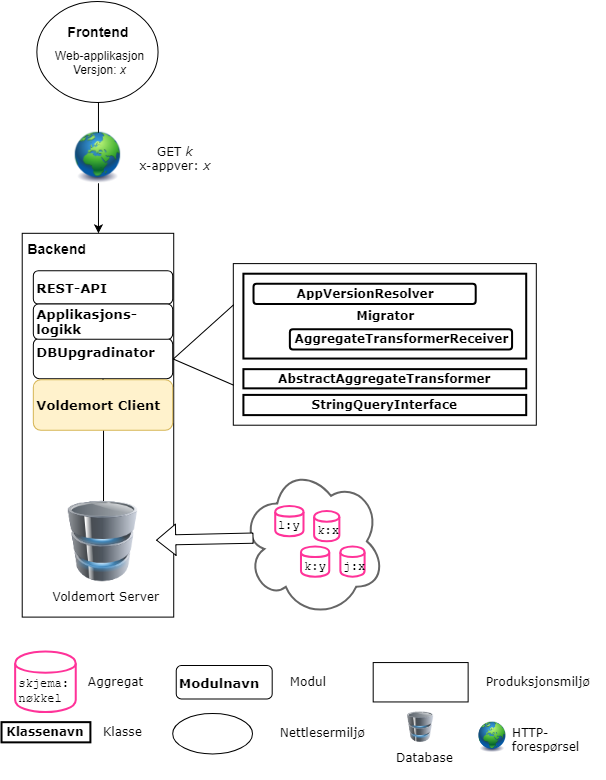
\includegraphics[scale=0.9]{fig/dbupgradinator-logisk-1.png}
    \caption{Logisk oversikt over moduler i det typiske produksjonsmiljøet DBUpgradinator opererer i. Klassene som DBUpgradinator består av nevnes med navn.}
    \label{fig5}
\end{figure}

% Figur 6
\begin{figure}[ht!]
    \centering
    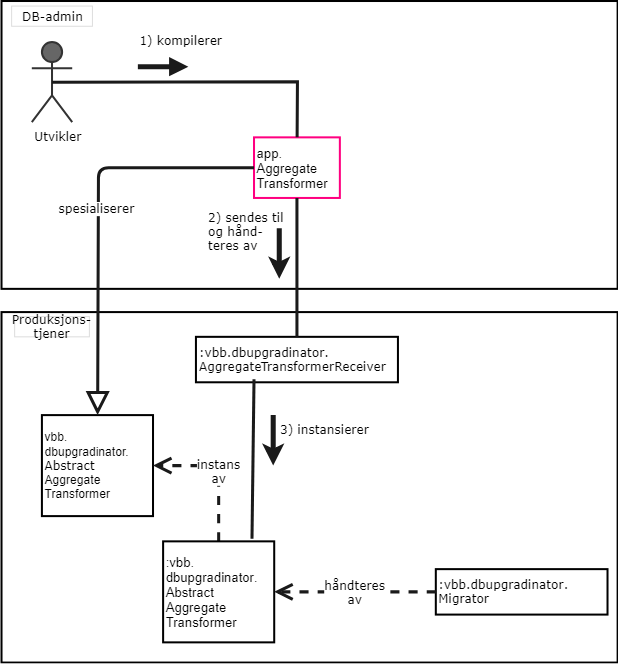
\includegraphics[scale=0.9]{fig/dbupgradinator-logisk-2.png}
    \caption{Logisk oversikt over moduler i det typiske produksjonsmiljøet DBUpgradinator opererer i. Klassene som DBUpgradinator består av nevnes med navn.}
    \label{fig6}
\end{figure}



\subsection{Det prosessmessige perspektiv}

\subsection{Det fysiske perspektiv}

